\documentclass[10pt,twocolumn]{article}
\usepackage[margin=0.75in]{geometry}
\usepackage{graphicx}
\usepackage{booktabs}
\usepackage{amsmath}
\usepackage{amssymb}
\usepackage{hyperref}
\usepackage{caption}
\captionsetup{font=small,labelfont=bf}
\setlength{\parskip}{3pt}
\setlength{\parindent}{0pt}

\title{\vspace{-3em}DSAI 490 -- Assignment 1\\Representation Learning with AE \& VAE on Medical MNIST}
\author{\small Ahmed Kahla}
\date{\vspace{-1em}}

\begin{document}
\maketitle
\vspace{-2em}

\section{Architectures}
Both the AE and VAE share a convolutional backbone on $64\!\times\!64$ grayscale inputs:
three strided $3\!\times\!3$ conv blocks ($32\!\to\!64\!\to\!128$ channels) followed by a dense
projection to a $D\!=\!16$ latent vector, and a mirrored transposed-conv decoder.
The \textbf{AE} produces a deterministic code $z=E(x)$ and minimizes mean-squared error
$\mathcal{L}_\text{AE} = \mathbb{E}\,\lVert x-D(z)\rVert^2$.
The \textbf{VAE} head instead outputs $(\mu,\log\sigma^2)$; a sample is drawn via the
reparameterization trick $z=\mu+\sigma\odot\varepsilon$ with $\varepsilon\sim\mathcal N(0,I)$.
Its objective combines a per-pixel binary cross-entropy and the Gaussian KL to the prior:
\[
\mathcal{L}_\text{VAE} = \underbrace{\mathbb{E}_{q(z|x)}[-\log p(x|z)]}_\text{recon}
 + \beta\,\underbrace{\mathrm{KL}(q(z|x)\,\|\,\mathcal N(0,I))}_\text{KL}.
\]
We linearly anneal $\beta$ from 0 to 1 over the first five epochs to avoid posterior collapse.

\section{Setup}
Medical MNIST (58k images, 6 classes) is streamed via \texttt{tf.data} with a fixed
$80/10/10$ train/val/test split per class. For each of the six anatomical regions we
train one AE and one VAE ($12$ models); we additionally train one \emph{global} AE and
one \emph{global} VAE on the union of all classes, used solely for the cross-class latent
visualization -- per-class encoders have unaligned latent axes, so stacking their codes
would produce a misleading plot. All models use Adam ($\text{lr}\!=\!10^{-3}$),
batch size~128, and 20~epochs. See \texttt{notebook.ipynb} for the full pipeline.

\section{Latent-space behavior}
\begin{figure}[h]
  \centering
  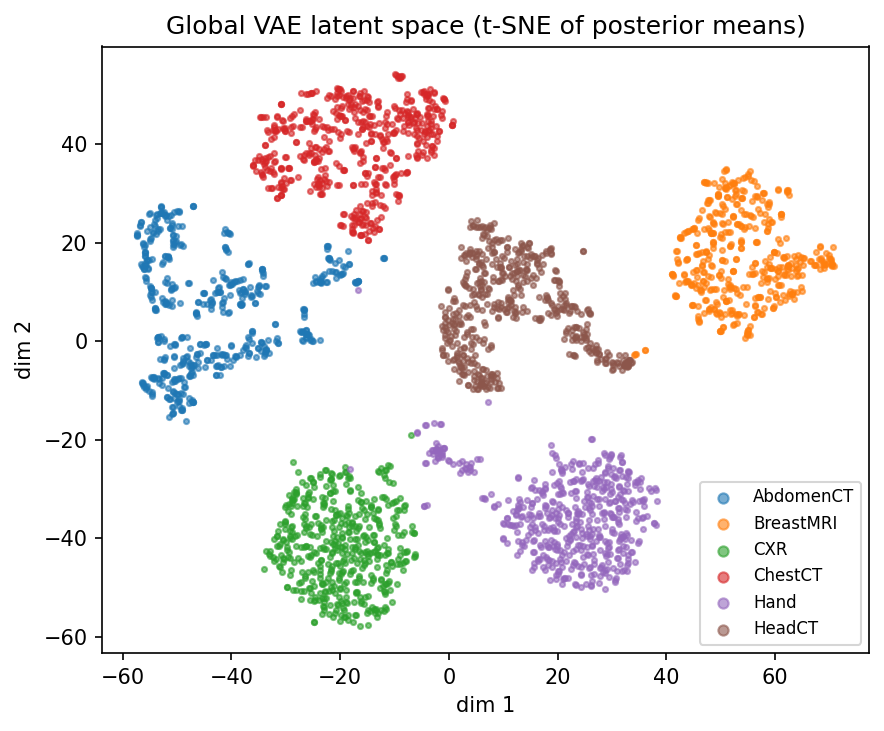
\includegraphics[width=\linewidth]{../figures/latent_vae_global_tsne.png}
  \caption{Global VAE latent space, t-SNE projection of posterior means on held-out data.
    Six anatomical regions form distinct but not isolated clusters, reflecting the smooth
    $\mathcal N(0,I)$ prior that is absent from the deterministic AE.}
  \label{fig:latent}
\end{figure}
The AE's latent space is compact but irregular: clusters are present but their relative
positions reflect arbitrary encoder geometry. The VAE's prior pulls codes toward
$\mathcal N(0,I)$, yielding a more continuous manifold where interpolating between
two codes decodes to a smooth morph between regions (see the latent-traversal figure in
\texttt{figures/}).

\section{Results}
\begin{figure}[h]
  \centering
  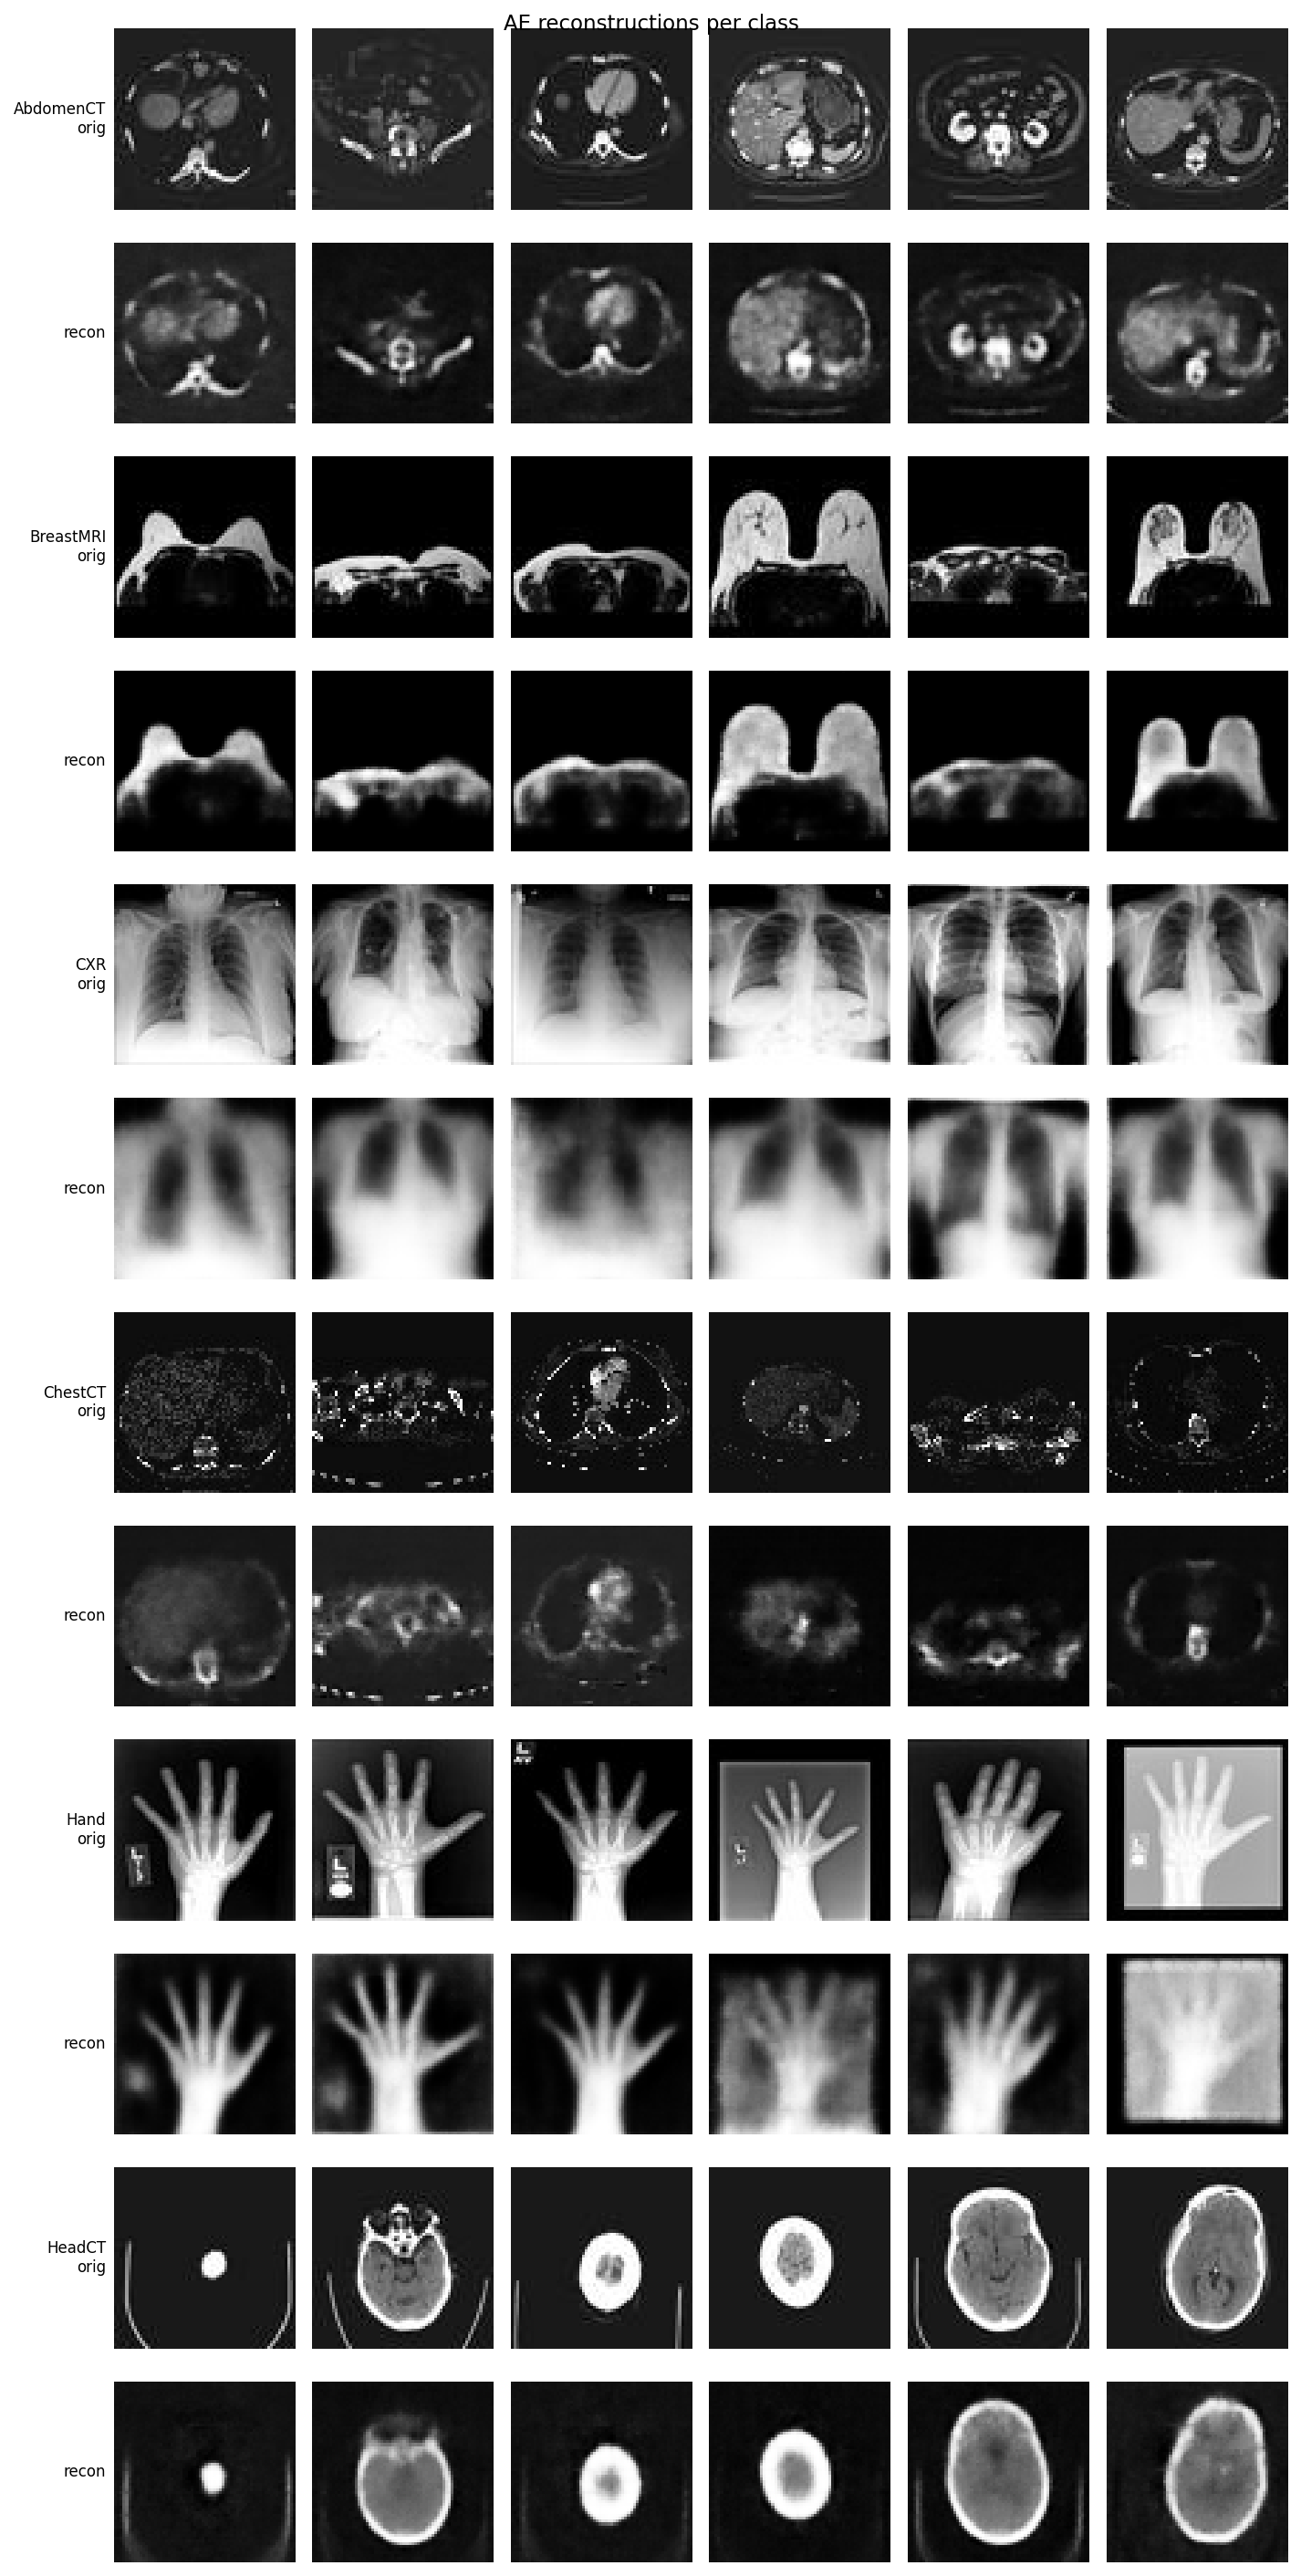
\includegraphics[width=\linewidth]{../figures/reconstructions_ae.png}\\[2pt]
  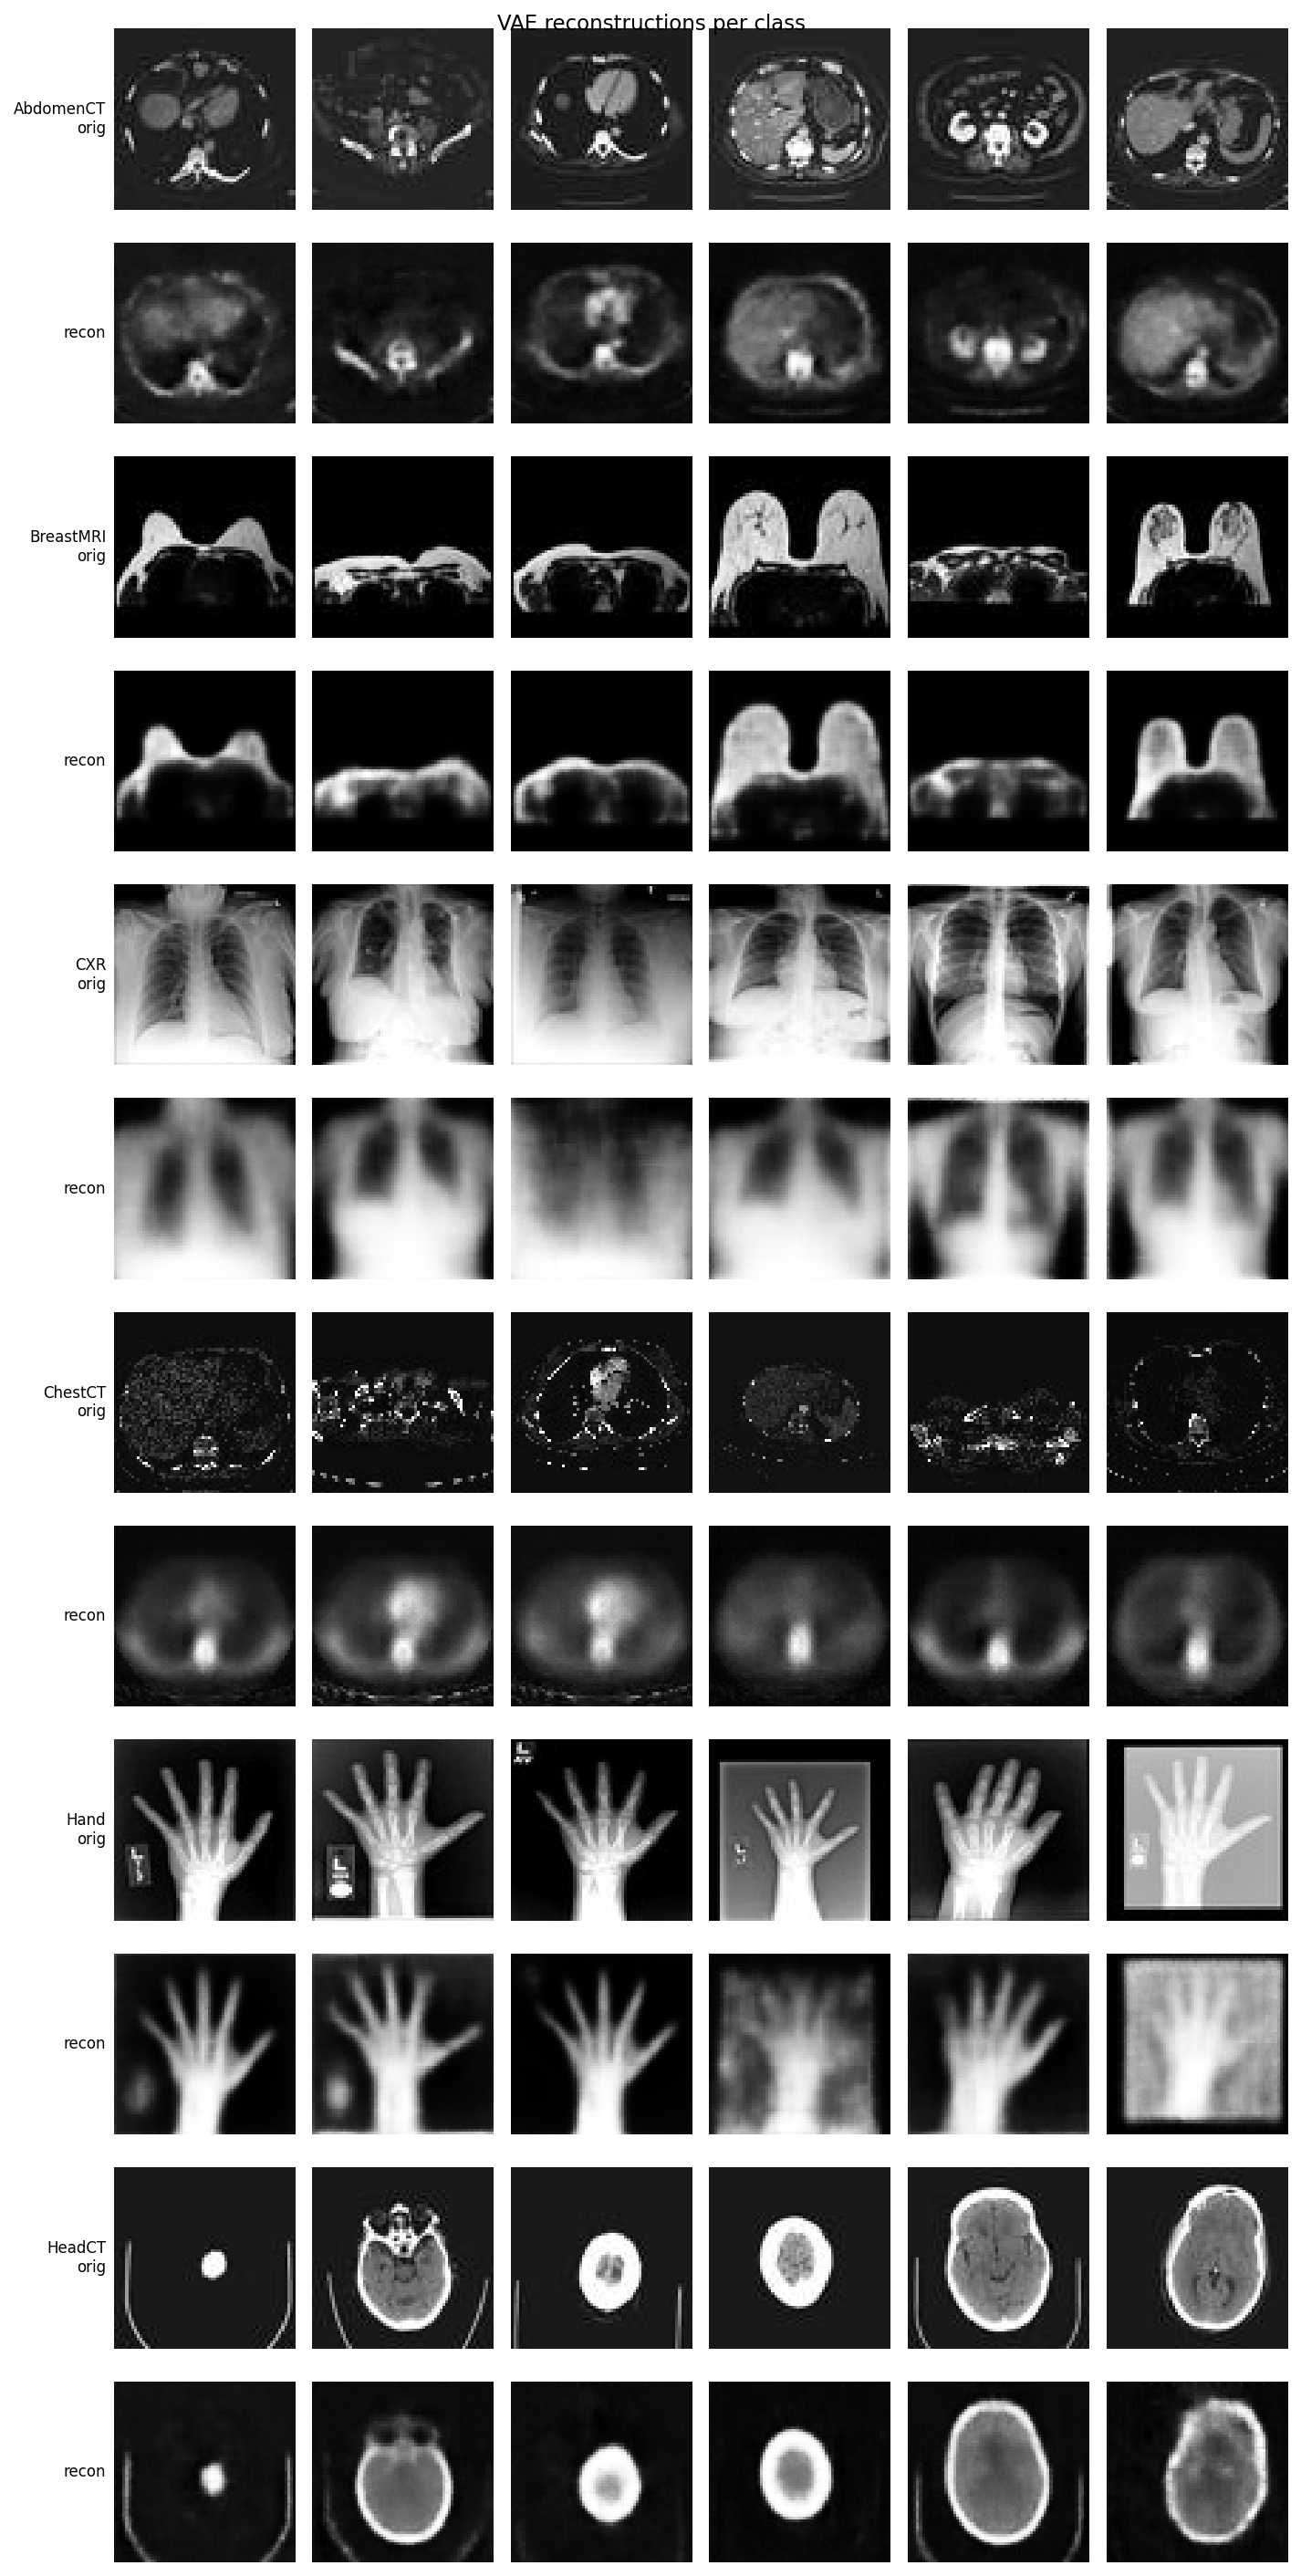
\includegraphics[width=\linewidth]{../figures/reconstructions_vae.png}
  \caption{Reconstructions per class. Top block: AE. Bottom block: VAE.
    Each pair shows originals above, reconstructions below.}
  \label{fig:recon}
\end{figure}

\begin{table}[h]
\centering\footnotesize
\begin{tabular}{lcccc}
\toprule
Class & AE MSE & AE SSIM & VAE MSE & VAE SSIM \\
\midrule
AbdomenCT & 0.0023 & 0.736 & 0.0038 & 0.637 \\
BreastMRI & 0.0060 & 0.751 & 0.0065 & 0.760 \\
CXR       & 0.0081 & 0.709 & 0.0090 & 0.693 \\
ChestCT   & 0.0023 & 0.643 & 0.0032 & 0.574 \\
Hand      & 0.0082 & 0.673 & 0.0095 & 0.680 \\
HeadCT    & 0.0103 & 0.706 & 0.0106 & 0.716 \\
\bottomrule
\end{tabular}
\caption{Test-set reconstruction metrics (fill from \texttt{figures/metrics\_per\_class.csv}).}
\label{tab:metrics}
\end{table}

As expected the AE produces sharper reconstructions (lower MSE, higher SSIM) because it
optimizes pixel fidelity directly, while the VAE trades a small amount of sharpness for
a structured latent that supports \emph{generation} from the prior (see
\texttt{figures/vae\_samples\_global.png}) and interpolation. For \emph{denoising},
both models improve on the noisy input at $\sigma\!\in\!\{0.1,0.2,0.3\}$; the VAE
degrades more gracefully at high $\sigma$ because its prior-regularized decoder resists
over-fitting to noise patterns.

\section{Insights}
KL warm-up was essential: without it, one or two classes drove the VAE into posterior
collapse within the first epoch. Per-region reconstruction difficulty ranks, roughly,
ChestCT $\approx$ AbdomenCT $<$ BreastMRI $<$ CXR $<$ Hand $<$ HeadCT (by AE MSE),
tracking intra-class variability. The cross-class t-SNE (Fig.~\ref{fig:latent}) confirms that the global
VAE's latent captures anatomical-region identity without any class supervision --
unsupervised representation learning is working as intended.

\end{document}
